\documentclass[a4paper,14pt]{extarticle}
\usepackage[utf8]{inputenc}
\usepackage[a4paper, lmargin=1cm, rmargin=1cm, tmargin=2cm, bmargin=3cm]{geometry}
\usepackage{multicol}
\usepackage{graphicx}
\usepackage{ulem}
\usepackage{scrextend}
% \usepackage[document]{ragged2e}


\newenvironment{Figure}
{\par\medskip\noindent\minipage{\linewidth}}
{\endminipage\par\medskip}

\setlength{\columnseprule}{0.5pt}
\pagestyle{empty}
\begin{document}
\makebox[.79\textwidth][r]{%
    \raisebox{-0.4\totalheight}[0pt][0pt]{%
    
\includegraphics[width=3.5cm]{bunny}
  }
}
\vspace{-1.1cm}
\begin{center}
    \Huge Pravila biljarda \textsc{Hiše Kolman}
\end{center}
\begin{multicols}{2}
    % \Large
    \begin{Figure}
    \centering
        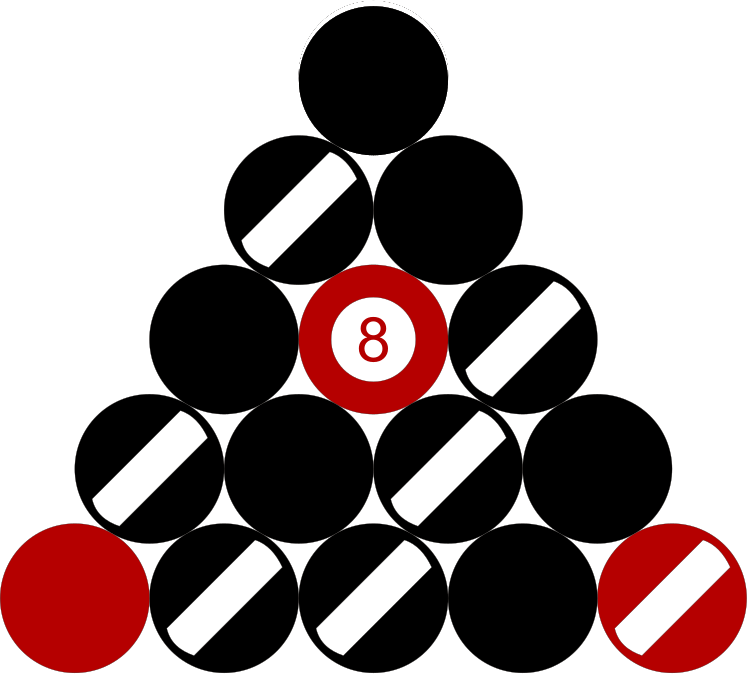
\includegraphics[width=.8\textwidth]{trikotnik.png}
        \vspace{-0.5cm}
    \end{Figure}
    \section{Začetna postavitev}
    \begin{enumerate}
        \item Pred prvim udarcem vse krogle postavimo v plastični trikotnik.
        \item Krogla št.~8 je na sredini trikotnika.
        \item Krogla št.~8 je nad označeno točko na mizi.
        \item V zadnjih dveh kotih trikotnika se morata nahajati ena polna in ena prazna krogla.
        \item Ostale krogle so razporejene poljubno.
    \end{enumerate}

    \section{Prvi udarec}
    \begin{enumerate}
        \item Prvi igralec je tisti, ki prejšnjo igro izgubil, ali pa se ta določi z žrebom ali obojestranskim dogovorom.
        \item Prvi igralec izbija belo kroglo iz označene točke na biljardu, ki je na drugi polovici mize, kot ostale krogle.
        \item Igralec mora s prvim udarcem vsaj štiri krogle, ki niso bela, zadeti ob rob mize. V nasprotnem primeru lahko njegov nasprotnik:
        \begin{enumerate}
            \item ponovno postavi trikotnik in on prevzame prvi udarec,
            \item ponovno postavi trikotnik in pusti, da prvi igralec ponavlja udarec,
            \item sprejme postavitev krogel in nadaljuje z igro.
        \end{enumerate}
        \item Če igralec s prvim udarcem pospravi kroglo št.~8, zmaga.
    \end{enumerate}

    \section{Pravila igre}
    \begin{enumerate}
        \item Igralca izmenično s palico udarjata belo kroglo in z njo poskušata pospraviti svoje barvne krogle.
        \item Vsak igralec si lasti bodisi prazne bodisi polne krogle. Prvi igralec, ki pospravi katero izmed barvnih krogel, si lahko izbere eno izmed barv pospravljenih krogel kot svojo.
        \item Vsakič, ko igralec naredi napako se njegova poteza zaključi. Njegov nasprotnik lahko postavi belo žogo na katerokoli mesto na mizi.
        \item Igralec mora pospraviti vse svoje krogle in nato še kroglo št.~8.
        \item Pred vsakim udarcem, s katerim želi pospraviti kroglo št.~8, mora igralec napovedati v katero luknjo jo bo pospravil.
    \end{enumerate}

    \section[Seznam napak]{Seznam napak\footnote{\label{hard_mode}Nekatera pravila so težja in se uveljavlja zgolj, ko se vsi udeleženi strinjajo z njimi.}}
    \begin{enumerate}
        \item Igralec pospravi belo kroglo.
        \item Igralec pospravi nasprotnikovo kroglo (razen v primeru, da igralca pred tem udarcem še nista imela dodeljenih barv krogel, npr.~s prvim udarcem pospravi eno polno in eno prazno kroglo).
        \item Igralec z belo zadane nasprotnikovo kroglo, ne da bi se bela prej odbila od roba ali kakšne njegove krogle.
        \item Igralec z udarcem izbije katerakoli kroglo iz mize. Krogle, ki so padle iz mize se smatrajo kot pospravljene.
        \item Igralec dvigne belo kroglo v zrak z udarcem pod težiščem. Kroglo se sme dvigovati samo z udarcem od zgoraj.
        \item Igralec se dotakne kakšne od krogel s čim drugim, kot konico palice.
        \item[$\star$\footref{hard_mode}] \textit{\emph{Igralec pospravi kroglo v luknjo, ki je ni napovedal.}}
        \item[$\star$\footref{hard_mode}] \textit{\emph{Igralec z belo kroglo najprej zadane nasprotnikovo ali črno kroglo (tudi z odboji od roba).}}
        \item[$\star$\footref{hard_mode}] \textit{\emph{Igralec z belo kroglo ne zadane svoje krogle.}}
        \item[$\star$\footref{hard_mode}] \textit{\emph{Po prvem trku med kroglami se nobena krogla ne dotakne roba mize.}}
    \end{enumerate}

    \section{Takojšnja izguba}
    \begin{enumerate}
        \item Igralec z belo zadane kroglo št.~8, ne da bi se bela prej odbila od roba ali kakšne njegove krogle.
        \item Igralec pospravi kroglo št.~8 preden je pospravil vse svoje ostale krogle.
        \item Igralec pospravi kroglo št.~8 v luknjo, ki je ni napovedal.
        \item Igralec pospravi kroglo št.~8 in belo kroglo z istim udarcem.
        \item Igralec izbije kroglo št.~8 iz mize.
        \item Igralec trikrat zaporedoma ne zadane nobene svoje krogle.
        \item[$\star$\footref{hard_mode}] \textit{\emph{Igralec trikrat (kumulativno) ne zadane krogle št.~8, ko je to še njegova edina krogla.}}
    \end{enumerate}
\end{multicols}

\end{document}
